% Minimal TikZ standalone example
\documentclass[tikz, border=1mm]{standalone}
%\usepackage[usenames,x11names,table]{xcolor}
% ----------------------------------------------------------------------
% Pour les images
%\usepackage{tikz}
\usetikzlibrary{calc,shadows,arrows,shapes,patterns,matrix}
\usetikzlibrary{decorations.pathmorphing}
\usetikzlibrary{fadings}
\usetikzlibrary{external}
\usetikzlibrary{positioning}
\usetikzlibrary{arrows}
\usetikzlibrary{backgrounds}
% Figure after Kjell Magne Fauske
% http://www.texample.net/tikz/examples/neural-network/
\begin{document}

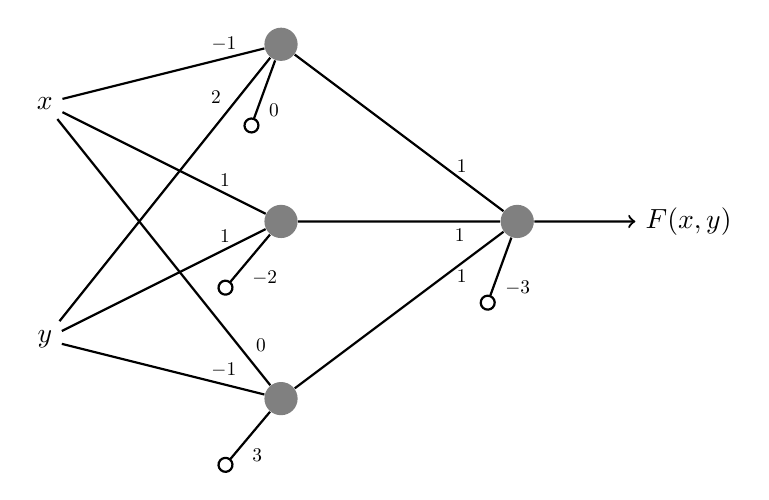
\begin{tikzpicture}[scale=1.5]
   \def\layersep{2cm}
    \tikzstyle{every pin edge}=[thick]
    \tikzstyle{neuron}=[circle,fill=black!25,minimum size=12pt,inner sep=0pt]
    \tikzstyle{entree}=[];
    \tikzstyle{input neuron}=[neuron, fill=black!50];
    \tikzstyle{output neuron}=[neuron, fill=black!50];
    \tikzstyle{hidden neuron}=[neuron, fill=black!50];
    \tikzstyle{annot} = [text width=4em, text centered]

% Entree
\node[entree] (E-1) at (-\layersep,-0.5) {$x$};
\node[entree] (E-2) at (-\layersep,-2.5) {$y$};

% Premiere couche
\node[input neuron] (I-1) at (0,0) {};
\node[input neuron] (I-2) at (0,-1.5) {};
\node[input neuron] (I-3) at (0,-3) {};

\node[below right=0.8ex,scale=0.7] at (I-1) {};
\node[below right=0.8ex,scale=0.7] at (I-2) {};
\node[below right=0.8ex,scale=0.7] at (I-2) {};

% \node[above right=0.8ex,blue] at (I-1) {$s_1$};
% \node[above right=0.8ex,blue] at (I-2) {$s_2$};
% \node[above right=0.8ex,blue] at (I-3) {$s_3$};

%Seconde couche et sortie
\node[output neuron] (O) at (\layersep,-1.5 cm) {};
\node[below right=0.8ex,scale=0.7] at (O) {};

% Arrete et poids
 \path[thick] (E-1) edge node[pos=0.8,above,scale=0.7]{$-1$} (I-1) ;
 \path[thick] (E-2) edge node[pos=0.8,above left,scale=0.7]{$2$} (I-1);
\draw[-o,thick] (I-1) to node[midway,below right,scale=0.7]{$0$} ++ (-110:0.8);

 \path[thick] (E-1) edge node[pos=0.8,above,scale=0.7]{$1$} (I-2);
 \path[thick] (E-2) edge node[pos=0.8,above,scale=0.7]{$1$} (I-2);
 \draw[-o,thick] (I-2) to node[midway,below right,scale=0.7]{$-2$} ++ (-130:0.8);

 \path[thick] (E-1) edge node[pos=0.9,above right,scale=0.7]{$0$} (I-3);
 \path[thick] (E-2) edge node[pos=0.8,above,scale=0.7]{$-1$} (I-3);
 \draw[-o,thick] (I-3) to node[midway,below right,scale=0.7]{$3$} ++ (-130:0.8);

 \path[thick] (I-1) edge node[pos=0.8,above,scale=0.7]{$1$} (O);
 \path[thick] (I-2) edge node[pos=0.8,below,scale=0.7]{$1$}(O);
 \path[thick] (I-3) edge node[pos=0.8,below,scale=0.7]{$1$}(O);
 \draw[-o,thick] (O) to node[midway,below right,scale=0.7]{$-3$} ++ (-110:0.8) ;

% Sortie
 \draw[->,thick] (O)-- ++(1,0) node[right]{$F(x,y)$};

\end{tikzpicture}  

\end{document}